\documentclass{article}
\usepackage{tikz}
\usepackage{float}
\usepackage{graphicx}
\usepackage{hyperref}
\usepackage[utf8]{inputenc}
\usepackage{enumitem}
\usepackage{listings}
\usepackage{xcolor}
\usetikzlibrary{shapes,arrows,positioning,fit,mindmap,trees}

\definecolor{lightgray}{RGB}{240,240,240}
\definecolor{primary}{RGB}{66,139,202}

\tikzstyle{block} = [rectangle, draw, fill=primary!20, 
    text width=8em, text centered, rounded corners, minimum height=4em]
\tikzstyle{line} = [draw, -latex']
\tikzstyle{cloud} = [draw, ellipse, fill=primary!20, 
    text width=8em, text centered, minimum height=4em]

\title{NexaApply: An AI-Powered Automated Job Application Form Filler for Web Platforms}
\author{Shovon Saha}
\date{\today}

\begin{document}

\maketitle

\begin{abstract}
NexaApply is a Chrome extension that utilizes artificial intelligence to automate the detection and completion of job application forms on various web platforms. By analyzing form structures and mapping fields to user-provided profiles, NexaApply streamlines the application process, reducing manual effort and minimizing errors. The extension ensures user data privacy by storing all information locally and offers customization options for enhanced user control.
\end{abstract}

\section{Background}
The job application process is often cumbersome and time-consuming, requiring applicants to repeatedly enter similar information across multiple platforms. This repetitive task not only leads to inefficiency but also increases the likelihood of errors, potentially affecting the success of applications. Existing solutions offer basic form-filling capabilities but lack intelligent field recognition and customization, limiting their effectiveness in diverse application environments.

\section{Summary}
NexaApply is a sophisticated Chrome extension designed to automate the job application process by intelligently detecting form fields on job portals and auto-filling them with user-specific profile information. Leveraging advanced AI algorithms, NexaApply analyzes form structures, matches fields with relevant user data, and ensures accurate and efficient form completion. The extension prioritizes user data privacy by maintaining all information locally and provides customizable settings to cater to individual user preferences.

\section{Detailed Description}
NexaApply integrates seamlessly with popular web browsers to provide users with an automated solution for filling out job application forms. Upon activation, the extension scans the current webpage for form elements, identifies relevant fields using the **FormAnalyzer** module, and maps them to the user's profile data stored locally. The **MistralAI** component enhances this process by analyzing the context and semantics of each field to ensure accurate data mapping.

Key Features:
- **Intelligent Field Detection:** Utilizes AI to recognize and categorize form fields accurately.
- **Customizable Profiles:** Allows users to input and manage their personal and professional information, which NexaApply uses to auto-fill applications.
- **Data Privacy:** Ensures all user data is stored securely on the local device, with encryption for sensitive information like API keys.
- **Debug Mode:** Provides detailed logs and real-time feedback to assist users in troubleshooting any issues during the auto-fill process.
- **Flexible Configuration:** Users can enable or disable features, adjust auto-fill settings, and manage their profiles through an intuitive options interface.

By automating repetitive tasks, NexaApply not only saves users valuable time but also enhances the accuracy of job applications, thereby increasing the chances of success in the competitive job market.

\section{Claims}
1. A Chrome extension named NexaApply that detects job application forms on web pages and automatically fills them using artificial intelligence to map form fields to user-provided profile data.

2. The extension of claim 1, wherein user profile information is stored locally on the user's device and encrypted to ensure data security.

3. The extension of claim 1, further comprising a debug mode that logs actions and errors to assist users in troubleshooting the auto-fill process.

4. The extension of any preceding claim, wherein the artificial intelligence analyzes field labels, types, IDs, and contextual information to determine the appropriate mapping of fields.

5. The extension of any preceding claim, wherein the extension supports multiple languages to accommodate international job application forms.

6. The extension of any preceding claim, wherein users can customize auto-fill settings, including enabling or disabling specific features and adjusting delay times between form submissions.

7. The extension of any preceding claim, wherein the extension integrates with the Mistral AI API to enhance form analysis and field matching accuracy.

8. The extension of any preceding claim, wherein the extension provides real-time feedback to users upon successful or failed auto-fill operations.

\section{Diagrams}

\subsection{Architectural Overview}

\begin{figure}[H]
    \centering
    \begin{tikzpicture}[node distance=2cm]

        % Nodes
        \node (user) [component] {User};
        \node (popup) [component, below of=user] {Popup Interface};
        \node (background) [component, below of=popup] {Background Service Worker};
        \node (content) [component, right of=background, xshift=3cm] {Content Scripts};
        \node (ai) [component, below of=background] {Mistral AI API};
        \node (storage) [component, left of=background, xshift=-3cm] {Local Storage};
        
        % Arrows
        \draw [arrow] (user) -- (popup) node[midway, left] {Interacts};
        \draw [arrow] (popup) -- (background) node[midway, left] {Sends Messages};
        \draw [arrow] (background) -- (content) node[midway, above] {Injects Scripts};
        \draw [arrow] (content) -- (background) node[midway, below] {Sends Data};
        \draw [arrow] (background) -- (ai) node[midway, right] {API Requests};
        \draw [arrow] (background) -- (storage) node[midway, above] {Reads/Writes};
        \draw [arrow] (ai) -- (background) node[midway, right] {API Responses};
        \draw [arrow] (content) -| (ai) node[pos=0.75, right] {Data Flow};

    \end{tikzpicture}
    \caption{Architectural Overview of NexaApply}
    \label{fig:architecture}
\end{figure}

\subsection{Workflow Diagram}

\begin{figure}[H]
    \centering
    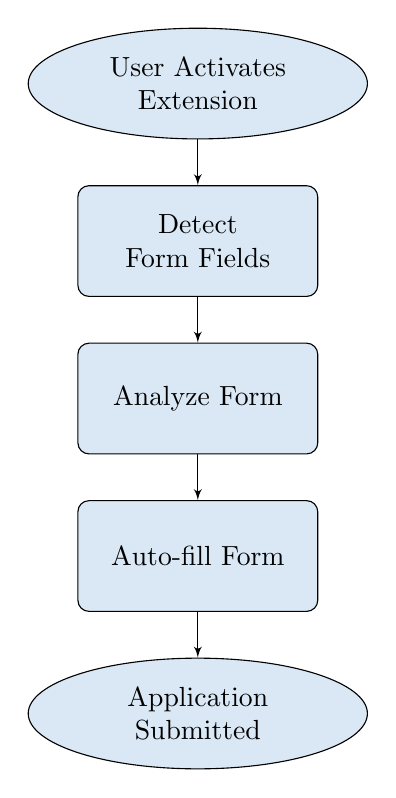
\begin{tikzpicture}[node distance=2cm, auto]
        \node [cloud] (start) {User Activates Extension};
        \node [block, below of=start] (detect) {Detect Form Fields};
        \node [block, below of=detect] (analyze) {Analyze Form};
        \node [block, below of=analyze] (fill) {Auto-fill Form};
        \node [cloud, below of=fill] (end) {Application Submitted};
        
        \path [line] (start) -- (detect);
        \path [line] (detect) -- (analyze);
        \path [line] (analyze) -- (fill);
        \path [line] (fill) -- (end);
    \end{tikzpicture}
    \caption{Workflow of NexaApply Extension}
    \label{fig:workflow}
\end{figure}

\subsection{Class Diagram}

\begin{figure}[H]
    \centering
    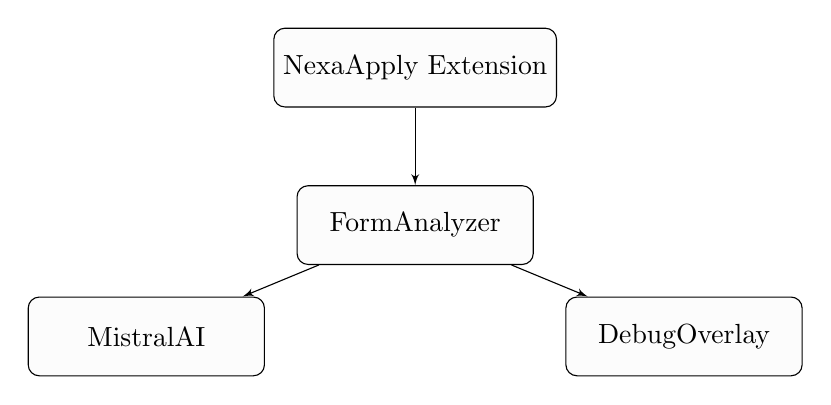
\begin{tikzpicture}[node distance=2cm, auto, class/.style={rectangle, draw, fill=lightgray!20, rounded corners, text centered, minimum width=3cm, minimum height=1cm}]
        \node[class] (NexaApply) {NexaApply Extension};
        \node[class, below of=NexaApply] (FormAnalyzer) {FormAnalyzer};
        \node[class, below left of=FormAnalyzer, xshift=-2cm] (MistralAI) {MistralAI};
        \node[class, below right of=FormAnalyzer, xshift=2cm] (DebugOverlay) {DebugOverlay};
        
        \path [line] (NexaApply) -- (FormAnalyzer);
        \path [line] (FormAnalyzer) -- (MistralAI);
        \path [line] (FormAnalyzer) -- (DebugOverlay);
    \end{tikzpicture}
    \caption{Class Diagram of Core Components}
    \label{fig:classdiagram}
\end{figure}

\end{document}
